\section{Introduction}

% To do:
% 1. American researchers: Yang punya property 1, 2, 3, dst itu mereka punya property apa?
% 2. [DONE] Outlier & sample size effect thd gini?
% 3. [DONE] Cek perbedaan 2 entitas di Introduction (pakai query difference) --> + Introduction

% %% include motivating scenario

% (tambahkan 2 paragraf pembukaan)
% distinct - minus = apa yang ada di NYC tapi ga ada di Batam
% Kasih contoh:
% 1. Entitas dengan tipe sama
% 2. Tunjukkan adanya singevalue vs multivalue
% 3. Tunjukkan adanya presence vs absence
% 4. Tunjukkan adanya incoming vs outgoing (incoming itu ga kalah penting, bisa jadi outgoing rendah tapi incoming nya banyak di refer entitas lain)
% 5. Tunjukkan adanya prop type

% contoh lain:
% 1. yang incomingnya banyak
% 2. yang external ID banyak

% Poin:
% 1. ...
% 2. ...

\begin{figure}[!htbp]
    \centering
    % 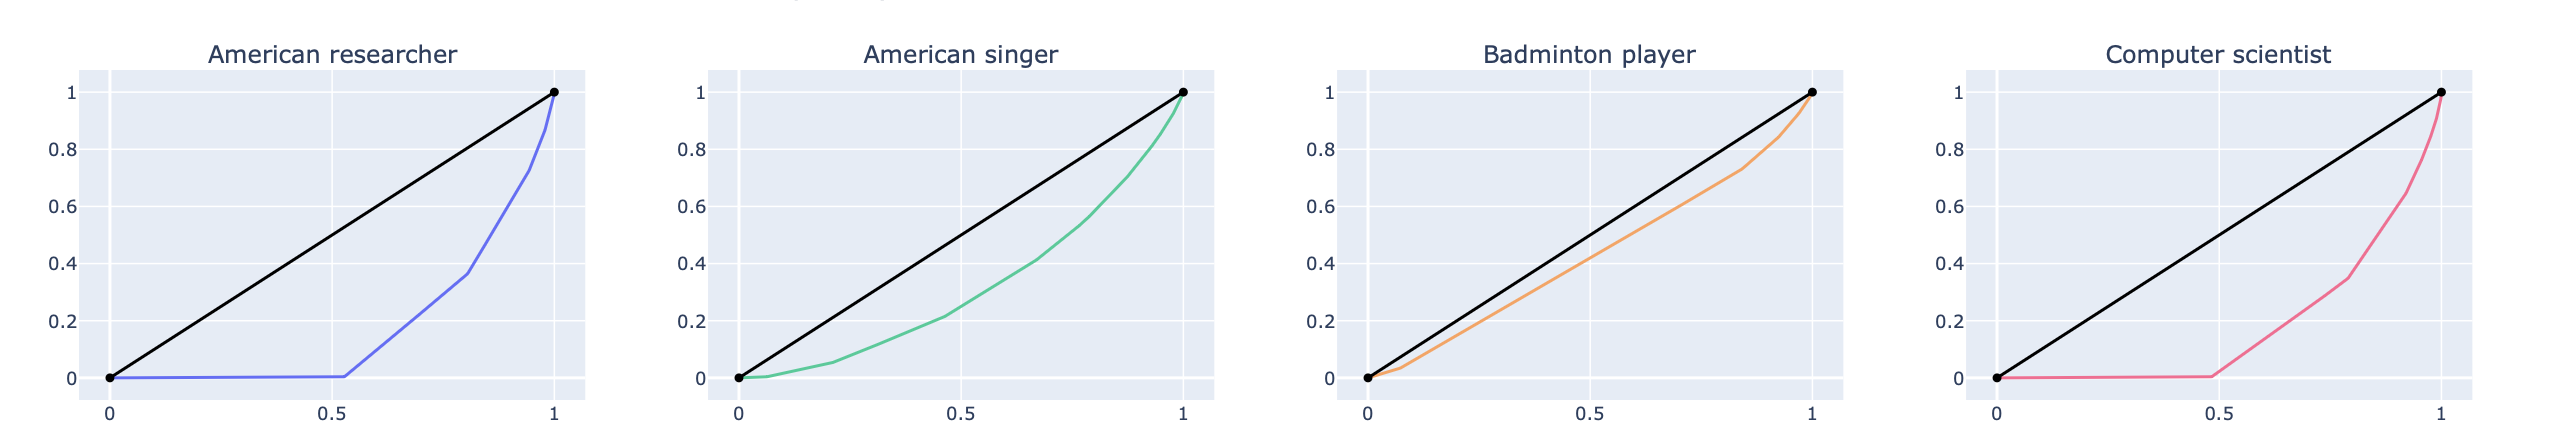
\includegraphics[scale=.5]{Gini - Pure Literal}
    \makebox[\textwidth][c]{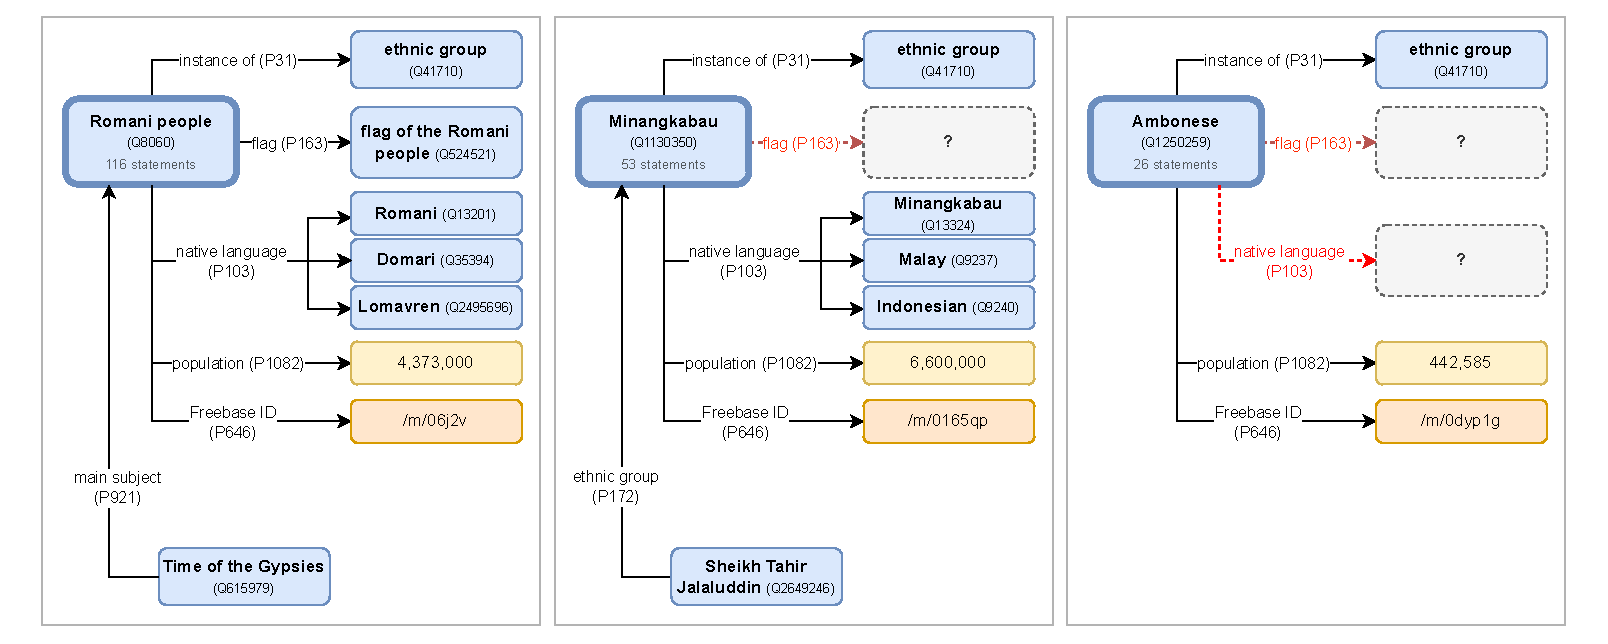
\includegraphics[width=1\textwidth]{Introduction - Wikidata 2}}%
    \caption{Data on Wikidata about the Romani people, the Minangkabau, and the Ambonese} \label{fig:intro-wikidata}
\end{figure}

Wealth is an abundance of valuable material possessions or resources. In economics, wealth is defined as an accumulation of valuable economic resources that can be measured in terms of either real goods or monetary value. When considering individual (human) wealth, the most common measure is net worth. On the other hand, in knowledge graphs (KGs), wealth can be defined as the amount of information (in terms of properties or links) an entity possesses.

\autoref{fig:intro-wikidata} shows three Wikidata entities of the type ethnic group: the Romani people, the Minangkabau, and the Ambonese, along with some information about them. For example, the entity Romani people includes information such as its class, flag, native languages, population, and associated Freebase ID. We can observe that a type of information can have a single value, such as the property \textit{flag} for each entity, which is exactly one (or zero, if the information does not exist), or multiple value, such as the property \textit{native languange}. Both of these properties have values that are other Wikidata entities. Additionally, there are other types of properties, such as \textit{population}, which has a static numerical value, and \textit{Freebase ID}, which provides a string used to identify the entity in the Freebase database.

While the previous examples focus on information with outgoing links, we can also consider the opposite perspective by examining incoming links. This approach does not directly show the possessions of an entity but rather indicates its popularity by showing how often it is mentioned elsewhere. This is illustrated by the Romani people being mentioned in \textit{Time of the Gypsies} and the Minangkabau being associated with Sheikh Tahir Jalaluddin.

The example in \autoref{fig:intro-wikidata} provides a clear picture of how entities in Wikidata can have different kinds and amounts of information, which may lead to knowledge imbalance. If this issue is left unaddressed, it can be problematic for anyone utilizing open KGs as a data source. Data users may draw invalid inferences and conclusions based on incomplete or imbalanced data, such as the Minangkabau and Ambonese are less important than the Romani. Moreover, if contributors to open KGs cannot identify which entities or classes are lacking information, efforts such as editathons may not be effective, potentially widening the gap between information-rich and information-poor entities. For example, contributors might prioritize enriching the Romani people's data while overlooking gaps in the Minangkabau entry, leaving the \textit{flag} property in the Minangkabau empty despite the well-documented existence of the Marawa flag of Minangkabau.

Existing approaches often focus on ...., lacking a way of quantifying the amount of information contained in KGs. Our study addresses this gap by proposing a formal model to define the knowledge wealth in the RDF knowledge graph. Additionally, we construct an analytical framework using statistical measures and visualization to give insights about the wealth of a class, the inequality between classes, and imbalance measure of wealth within a class. To evaluate this framework, we conducted several use cases on various classes in Wikidata.

Our contributions are:
\begin{enumerate}
    \item We introduce the 3 notions of quantifying knowledge wealth for knowledge graphs, and show how they can be used to further characterize knowledge wealth in knowledge graphs.
    \item We implemented the formal and insight model using Python programming language and made it accessible.
    \item We perform a case study on Wikidata classes, showing how biases can be identified in Wikidata, how different definition of wealth impacts the imbalance level of a class, and how the composisition of wealth based on is.
\end{enumerate}